\documentclass[10.5pt]{article}
\usepackage[margin=1.1in]{geometry}
\usepackage[utf8]{inputenc}
\usepackage{ amssymb }
\usepackage{amsmath}
\usepackage{mdframed}
\usepackage{minted}
\surroundwithmdframed[linewidth = 1pt]{minted}
\usepackage{parskip}
\usepackage{graphicx}
\usepackage{float}
\usepackage{fancyhdr}
\setlength{\headheight}{3cm}
\thispagestyle{fancy}
\renewcommand{\headrulewidth}{0pt}


\lhead{
\begin{minipage}{2.5cm}
\begin{figure}[H]

\includegraphics[width=2.5cm]{oie_logo.png}
\end{figure}
\end{minipage} 
\begin{minipage}{8cm}
\textbf{XXV Olimpiada Inform\'atica Espa\~nola}\\
Primer concurso clasificatorio\\
\texttt{cuadrados\_libreta}
\end{minipage}
}

\begin{document}



\section*{Cuadrados en la libreta}

La libreta de Juan es de esas que tienen pautas horizontales. En una p\'agina tiene $m$ l\'ineas horizontales, separadas cada una un cent\'imetro de la anterior. A Juan, sin embargo, le gustan las libretas que tienen pauta cuadriculada. Por ello, ha dibujado en una p\'agina de su libreta $n$ l\'ineas verticales en las coordenadas horizontales $a_1, a_2, \ldots, a_n$, es decir, la distancia de la $i$-\'esima l\'inea al borde izquierdo de la p\'agina es de $a_i$ cent\'imetros. Tanto las l\'ineas de pauta horizontal como las l\'ineas que ha dibujado Juan recorren toda la p\'agina.

Ahora Juan se pregunta cu\'antos cuadrados hay con v\'ertices en intersecciones entre las l\'ineas en la libreta. Ayuda a Juan a contar el n\'umero de cuadrados.


\subsection*{Entrada y salida}

La primera l\'inea de la entrada continene dos enteros $m$ y $n$. La segunda l\'inea contiene $n$ enteros $a_1, \ldots, a_n$.

La salida debe contener una \'unica l\'inea con el n\'umero de cuadrados.

\subsection*{Ejemplos}
\subsubsection*{Ejemplo 1}

Entrada:
\begin{minted}[obeytabs=true, breaklines, breakautoindent=true]{text}
4 3
1 3 4
\end{minted}
Salida:
\begin{minted}[obeytabs=true, breaklines, breakautoindent=true]{text}
6
\end{minted}

Con las $7$ rectas dibujadas se pueden formar $6$ cuadrados, tal como se muestra en la imagen.

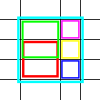
\includegraphics[width=2.5cm]{sample1.png}

\subsubsection*{Ejemplo 2}
Entrada:
\begin{minted}[obeytabs=true, breaklines, breakautoindent=true]{text}
2 2
1 2
\end{minted}
Salida:
\begin{minted}[obeytabs=true, breaklines, breakautoindent=true]{text}
1
\end{minted}

\subsubsection*{Ejemplo 3}
Entrada:
\begin{minted}[obeytabs=true, breaklines, breakautoindent=true]{text}
3 2
1 5
\end{minted}
Salida:
\begin{minted}[obeytabs=true, breaklines, breakautoindent=true]{text}
0
\end{minted}

\subsection*{Restricciones}
$2 \leq m \leq 10^6$.

$2 \leq n \leq 10^6$.

$1 \leq a_1 < a_2 < \ldots < a_n \leq 10^9$.
\subsection*{Subtareas}

\begin{enumerate}
    \item (14 puntos) $n, m, a_n \leq 100$.
    \item (25 puntos) $n \leq 2000$.
    \item (10 puntos) $m = 2$.
    \item (13 puntos) $a_i = i$ para $1 \leq i \leq n$.
    \item (38 puntos) Sin restricciones adicionales.
\end{enumerate}



\end{document}
